\subsubsection{Descripci\'on} 

Dado un conjunto de atrinutos \( M \) y un conjunto de implicaciones (o dependencias funcionales) \( \Sigma \) sobre \( M \) y sea \( X \subseteq M \), el cierre de \( X \) con respecto a \( \Sigma \), \( X^+_{\Sigma} \), es el subconjunto de \( M \) mas grande que cumple que \( \Sigma \vdash X \to X^+_{\Sigma} \).

El cierre es muy usado en inteligencia artificial y bases de datos, ya que es un punto clave en la resoluci\'on de muchos problemas: eliminaci\'on de restricciones redundantes, optimizaci\'on de consultas y el problema de la b\'usqueda de claves.

Por ello, se ha desarrollado un algoritmo de cierre basado en la l\'ogica de implicaciones, que en el peor de los casos, tiene la misma complejidad que los algoritmos de cierre lineales existentes.

De nuevo, se dispon\'ia de una primera implementaci\'on del algoritmo, la cual ha sido mejorada y optimizada con el fin de reducir el coste computacional del c\'alculo del cierre.

Si comparamos esta versi\'on del algoritmo con las principales versiones que podemos encontrar a lo largo de la literatura podemos ver que se consigue una mejora considerable:

\begin{center}
    \begin{tabular}{c c}
        \hline
        M\'etodo & Tiempo Medio (ms) \\
        \hline
        Diederich Closure & 4.593,48 \\   
        Beeri Closure & 7.013,56 \\   
        Paredaens Closure & 5.863,35 \\  
        SLFD -Closure & 1.262,41 \\  
    \end{tabular}
\end{center}
\newpage
\subsubsection{C\'odigo} 
\lstinputlisting{r_code/closure.R}
\subsubsection{Ejemplo} 
\begin{figure}[h]
    \centering
    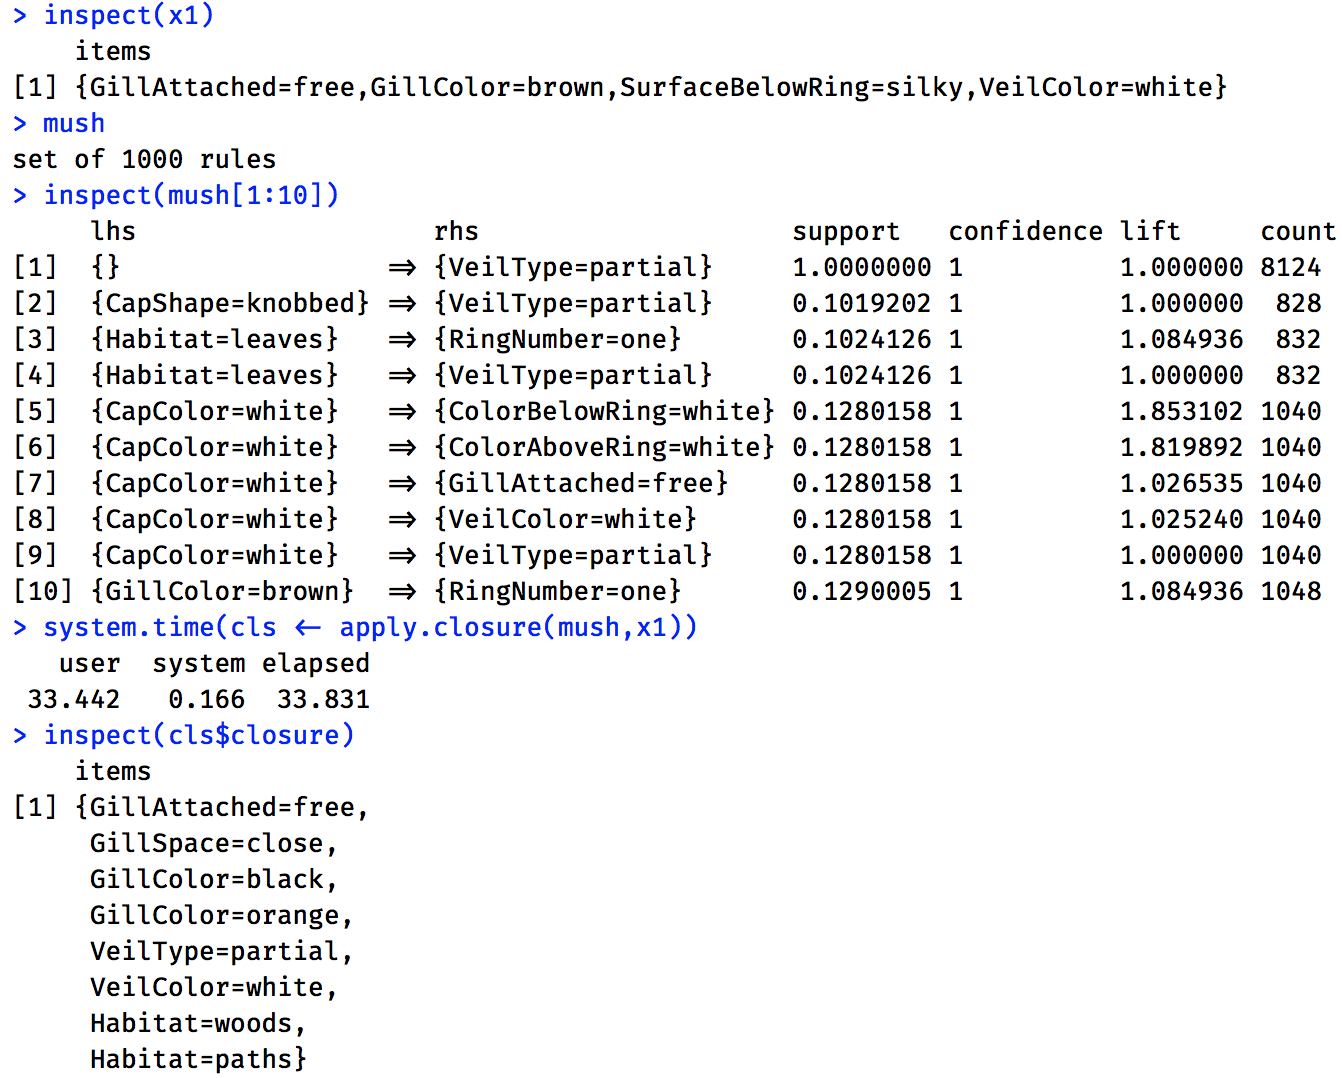
\includegraphics[scale=0.6]{closure_ejemplo}
    \caption{Ejemplo apply.closure}
    \label{fig:closure_ejemplo}
\end{figure} 

Como se puede ver, dado un conjunto de atributos (x1) y un conjunto de reglas (mush), en este caso de 1000 reglas, se puede calcular el cierre de x1 respecto a mush en tan solo 33 segundos, tiempo bastante bueno teniendo en cuenta el tama\~no del conjunto de reglas.
\subsubsection{Comparativa/Versiones} 

\begin{figure}[h]
    \centering
    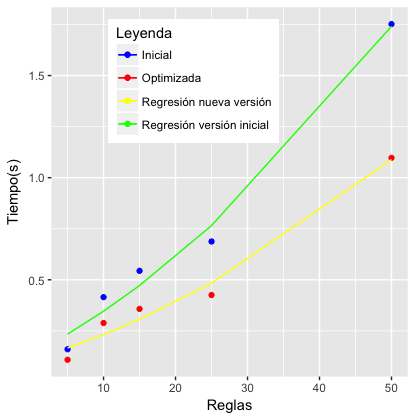
\includegraphics[scale=0.75]{closure}
    \caption{Pruebas apply.closure}
    \label{fig:closure}
\end{figure} 

En la figura \ref{fig:closure} se puede ver una gr\'afica comparativa entre dos versiones distintas de esta funci\'on. La primera de ellas es la versi\'on de la que dispon\'ia el director de este TFG en el momento en que se empez\'o a desarrollar el mismo. La segunda es una versi\'on mejorada (como se puede ver m\'as arriba en el extracto de c\'odigo), que se realiz\'o como parte de este trabajo.

En este caso, dado que el coste computacional de esta funci\'on no es demasiado grande, las diferencias de rendimiento tampoco lo son si el n\'umero de reglas no es demasiado grande.

